\documentclass{article}%
\usepackage[T1]{fontenc}%
\usepackage[utf8]{inputenc}%
\usepackage{lmodern}%
\usepackage{textcomp}%
\usepackage{lastpage}%
\usepackage[head=40pt,margin=0.5in,bottom=0.6in]{geometry}%
\usepackage{graphicx}%
%
\title{\textbf{El País: El olvido de los muertos en las protestas contra Nicolás Maduro}}%
\author{EL NACIONAL WEB}%
\date{16/09/2018}%
%
\begin{document}%
\normalsize%
\maketitle%
\textbf{URL: }%
http://www.el{-}nacional.com/noticias/sociedad/pais{-}olvido{-}los{-}muertos{-}las{-}protestas{-}contra{-}nicolas{-}maduro\_251949\newline%
%
\textbf{Periodico: }%
EN, %
ID: %
251949, %
Seccion: %
Sociedad\newline%
%
\textbf{Palabras Claves: }%
Sociedad\newline%
%
\textbf{Derecho: }%
1.10%
, Otros Derechos: %
5%
, Sub Derechos: %
1.10.1%
\newline%
%
\textbf{EP: }%
NO\newline%
\newline%
%
\textbf{\textit{El expediente de Juan Pablo Pernalete reposó durante meses en un cajón de la fiscalía en Caracas, hasta que sus padres y su abogado pudieron acceder a él por un cambio en la fiscal que llevaba el caso}}%
\newline%
\newline%
%
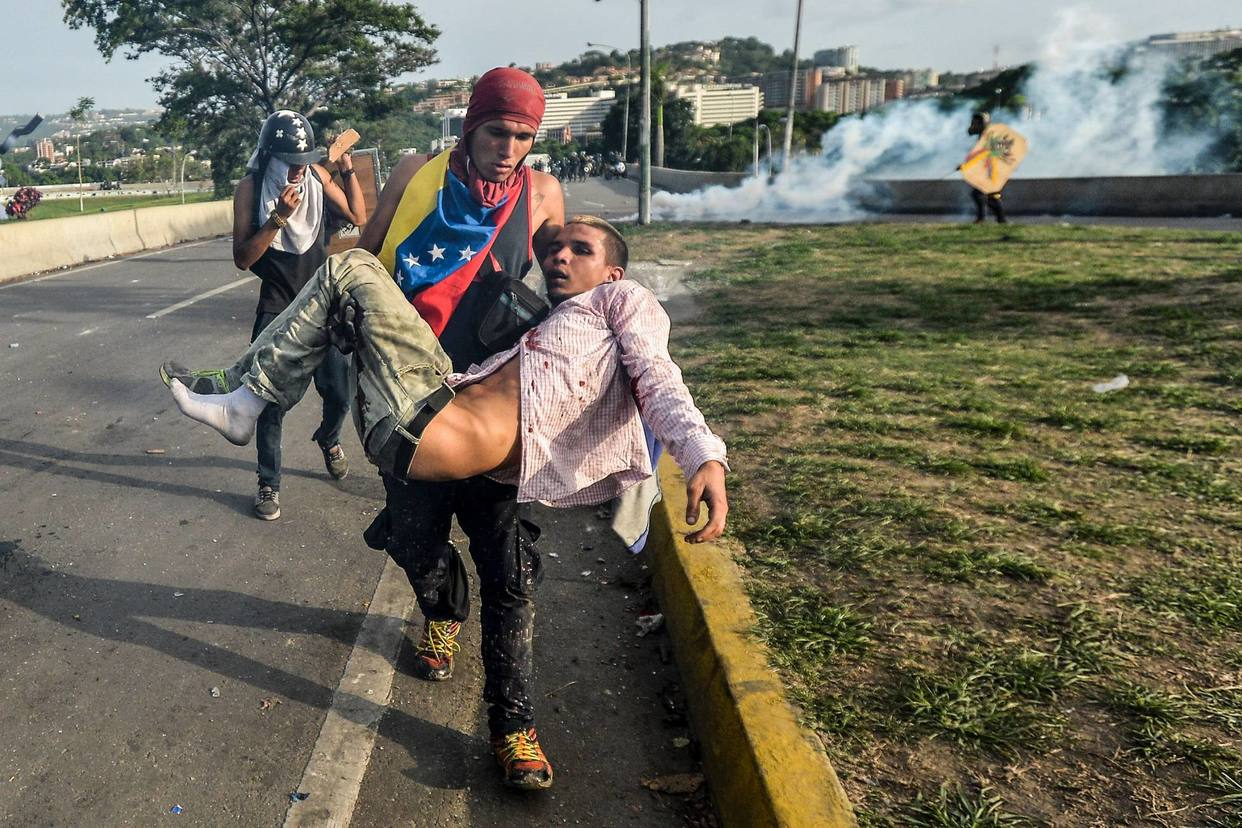
\includegraphics[width=300px]{64.jpg}%
\newline%
%
Durante los tres meses de protestas del 2017 fueron muchos los casos de jóvenes que murieron en manos de las autoridades. En ese sentido, Liliana Ortega, directora del Comité de Familiares de Víctimas, asegura que~98\% de las denuncias por violaciones de los derechos humanos de jóvenes manifestantes contra el régimen de Nicolás Maduro en Venezuela quedan sin investigar y no llegan a ser juzgadas.%
\newline%
%
Familiares de Juan Pablo Pernalete, uno de los estudiantes que asesinaron en la plaza Altamira, intentan desde hace meses desbloquear el proceso judicial del crimen de su hijo, reseñó~El País.%
\newline%
%
Días antes de la protesta, Maduro~había consolidado su autoritarismo al apoyar dos sentencias del Tribunal Supremo que eliminaron la inmunidad de diputados, suprimieron las funciones de la Asamblea Nacional y~lo facultaron para poder legislar;%
\newline%
%
El expediente de Juan Pablo, como el de tantos otros venezolanos, reposó durante meses en un cajón de la fiscalía de Caracas hasta que sus padres y su abogado pudieron acceder a él, luego de un cambio en la fiscal que llevaba el caso. El padre del joven asegura que el Ministerio Público ha pedido datos a la Guardia Nacional sobre el grupo que estuvo en Altamira el día que mataron a su hijo, pero el alto mando militar se niega a colaborar.%
\newline%
%
Otro caso del que tampoco se ha hecho justicia es el del asesinato de David Vallenilla, un estudiante de enfermería. A Vallenilla~le disparó un sargento de la Aviación cuando protestaba en la base aérea Generalísimo Francisco de Miranda.%
\newline%
%
Lea más en~El País.%
\newline%
%
\end{document}